\chapter{Results}\label{ch:results}
Real world tests proposed in chapter \ref{ch:method} are executed from within the network of Nikhef to the network of company x during a maintenance window.
For the methodology containing the use cases DPDK was used as a framework to find the limitations of the hardware in the path. 
Pktgen was used for T1 and T2. WARP was used to get the results for T3.
A combination of WARP and NGINX was used to get the results for T4. 

%From the experiments described in chapter \ref{ch:experiments} a framework was created and tested in chapter \ref{ch:method}. 
%The 'easy to use' tools like iPerf3, hping and BoNeSi are useful for quick tests. But when it comes to representative session based application testing these tools do not offer the solution for high speed networks. 
%As these 'easy to use' tools all require the kernel to talk to the hardware. As described in section \ref{sub:dpdk}, DPDK is able to bypass the kernel and talk to the interface directly. Cores and memory needs to be dedicated to generate traffic.  

\section{Infrastructure}
The network at company x as it is shown in figure \ref{fig:nikhefuva} is a simplified representation.
The detailed infrastructure used during the real world test is displayed in figure \ref{fig:companyx}. 
Since all the network hardware is redundant and a single device failure cannot result in total downtime the network and therefore the monitoring gets more complicated.
The server is connected to a data center layer that is spread over two physical locations, one serving as the active and the other as the passive environment.
To minimize broadcast traffic between the data centers an overlay technique is used. This overlay blocks broadcast storms at one location spreading to the other location.
During the tests we did not reach hardware limits based on capacity. 
Therefore, the overhead from the overlay technique is not a problem during these tests.  
The network is not in production and the server used for the tests is the only server connected to the data center switches.     
When traffic does not arrive at the destination, detailed measurements are needed at every device for every link to determine where the traffic gets dropped.   

\begin{figure}[H] 
  \includegraphics[scale=0.4]{images/companyx.pdf}
  \caption{Detailed visualization of real world scenario.}
  \label{fig:companyx}
\end{figure}

\section{Monitoring}\label{sec:monitoring}
During the test cases, we executed the tests while monitoring all of the interfaces used for the path from client to destination.
The experimental environment was monitored using the SNMP collector. SURFstat monitors the link utilization between Nikhef and company x. Company x used an SNMP collector to monitor all the links from the Internet Service Provider to the destination of the test.    
Interfaces from possible backup paths were monitored as well. 
Due to the complexity of the network, graphs displaying multiple links are created to present a total picture of the used bandwidth during the maintenance window.
Figures shown in this chapter display the graphs of the throughput that was sent out of the aggregated interfaces connecting router1 to the firewall cluster and the links connecting the firewalls to the DCI switches inside the data center. 
SURFstat provided figure \ref{fig:surftest} displaying the generated throughput between source and destination networks.
This figure is used to see if the measured incoming throughput was the same as the measured outgoing bandwidth from Nikhef's network.

\begin{center}
\begin{figure}[H]
  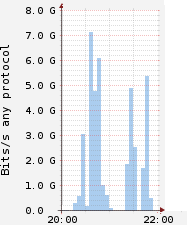
\includegraphics[scale=0.8]{images/test-link-usage.png}
  \caption{Bandwidth utilization of real world tests from Nikhef to company X during the time window the use cases were executed (figure provided by SURFstat).}
  \label{fig:surftest}
\end{figure}
\end{center}

\section{Data Plane Development Kit based tools}
The results of the DPDK based applications pktgen and WARP are explained during the performance tests in the real world scenario.
 
\subsection{pktgen}
Due to hashing algorithms used inside the core network of Nikhef, the real world test using pktgen could never reach more than 10Gb/s. 
The production network of Nikhef could not be altered during the tests. \\ 

The hashing algorithm used by the switch should be configured to divide the load coming in from the internal network. 
When most of the traffic is generated by one source to one destination using a single session, the throughput for a single flow will never reach above 10Gb/s in the network setup used during the tests.
Knowing the traffic patterns during the design phase of a network can overcome these issues.
Using multiple streams between client and server can improve the performance but this cannot be achieved using pktgen.
Multiple clients generating traffic towards one destination can fill the capacity of multiple links to reach 40Gb/s. \\

%DPDK and pktgen can be used to high bandwidth session based throughput testing. Limits can be reached up to layer 3 of the OSI model.

% 20:42 - 20:50 PKTGEN UDP en TCP
% 20:54 - 21:00 WARP - NGINX
% 21:21 - 21:30 WARP - RAW TCP
% 21:42 - 22:00 WARP - HTTP

\subsection{WARP}
From the benchmark results performed on WARP in chapter \ref{ch:experiments} it is known WARP is capable of generating a million session per second for raw TCP and HTTP requests. 
WARP was used to run three tests. WARP needs to be commanded using its own syntax. The command file that was used for the NGINX server test and the WARP HTTP server test can be found in appendix \ref{app:realworld}. As WARP runs on top of DPDK, the DPDK commands point to resources that will be claimed by DPDK. As an example:

\begin{verbatim}
./build/warp17 -c ff -n 4 -m 32768 -- --qmap-default max-c \
--tcb-pool-sz 32768 --cmd-file test-client-nginx-http.txt 
\end{verbatim} 

DPDK is started using 8 cores and 4 memory channels loading 32GB of memory, a default optimal mapping for CPU to NIC binding is chosen and the 32MB of memory is used per TCP control block size and a command file is used to start WARP.

Figure \ref{fig:warptime} shows the results of the three experiments executed with the use of WARP, to get the results for use cases three and four.
Measurements were taken at the interfaces used to handle the data from the client going into the network towards the destination during the three upcoming tests.
A first test where WARP was used to retrieve a 500 Kbyte file from an NGINX web server running on server A was executed. This NGINX server was tuned for performance \cite{nginxtuning}.
The file was placed on a RAM disk to make sure disk IO would not be the bottleneck during the performance tests. 
The first test is executed starting at 20:50 and it ran until 21:00. The request size is increased every 90 seconds with an interval of 30 seconds between the tests.
During this test the following request sizes where used: 64, 256, 512, 1024 and 2048 bytes. 
Figure \ref{fig:realnginx} shows that the amount of traffic leaving the server goes above 4Gb/s while only 0.6 Gb/s of requests are coming in on the receiving end. 
This matches the values shown in figure \ref{fig:warptime}. \\
A choice to rate limit at the NGINX server at the receiving end (allowing the server to accept a maximum of 50.000 concurrent sessions) was made to restrict the service from being overloaded by the client. Although the server was limited to 50.000 concurrent sessions, all the available sessions were used by WARP which made the service unavailable for other users.
This proves the infrastructure and the application are capable of handling 50.000 sessions.

\begin{figure}[H]
  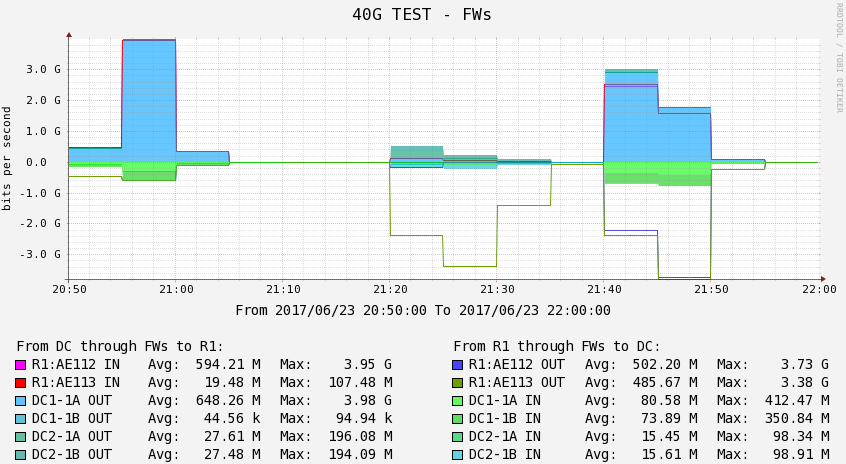
\includegraphics[scale=0.5]{images/warp-timeline.png}
  \caption{Time line of the performed tests using WARP displaying the bandwidth usage over time}
  \label{fig:warptime}
\end{figure}

\begin{figure}[H]
  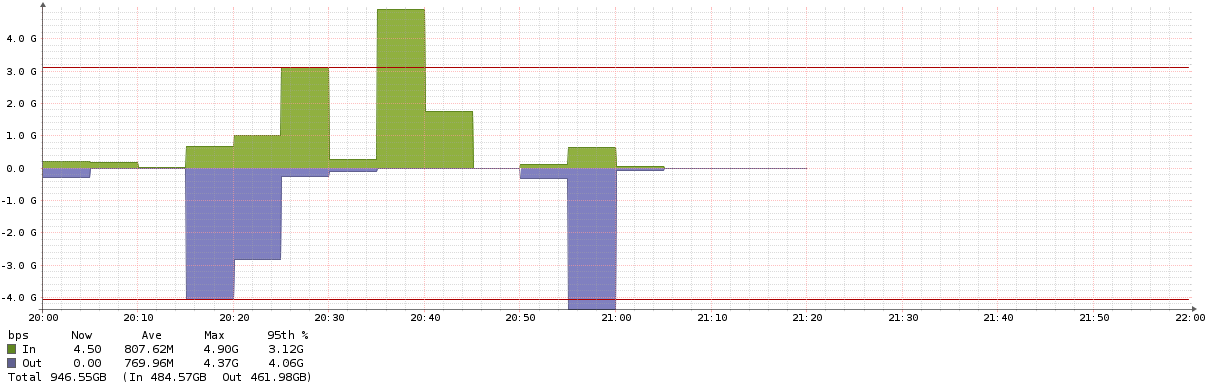
\includegraphics[scale=0.35]{images/real-nginx.png}
  \caption{Bandwidth utilization server A during NGINX test, measurements from servers perspective }
  \label{fig:realnginx}
\end{figure}

At 21:20 test 2 was started, to determine the limitation of handling layer 4 data as detailed in paragraph \ref{sub:t4real}.
Generating a maximum amount of raw TCP session from client to server both running WARP and using 32GB of memory and all cores to generate traffic.
Request and response sizes chosen for this tests are: 64, 256, 512, 1024 and 2048 bytes. 
The bandwidth utilization measurements are from the uplink and downlink interfaces of the devices in the path as shown in figure \ref{fig:companyx} represented by "AE112" and "AE113".
Two separate graphs are displayed for these links, figure \ref{fig:testrealusageae112} shows all the interfaces connected to firewall1 and figure \ref{fig:testrealusageae113} shows all the interfaces connected to firewall2.
The graphs display traffic that went out of one interface and is expected to come into the interface at the other side when the firewall forwards the traffic, when this does not happen white gaps can seen as marked with the red arrow in figure \ref{fig:testrealusageae112}. 
The blue line represents data that left the router interface and the green bar represent the data that was received by the data center switches. 
These white gaps in the graph represent the data that got lost due to failing hardware during the execution of the tests. 
Data points above zero represent data that went from server to client and data points below zero represent data from client to server.  
 
Firewall sessions statistics were not registered due to logging problems in the firewall environment that we were not able to repair before the end of the maintenance window. 
Chapter \ref{ch:experiments} shows that the benchmark value of 1 million sessions per second can be generated, where only small differences are observed at different packets sizes. 
The graph in figure \ref{fig:testrealusageae112} doesn't display any traffic at the start of this second test at 21:20. This is the moment the raw TCP test was started while figure \ref{fig:surftest} displays traffic towards the tested network. 
 
\begin{figure}[H]
  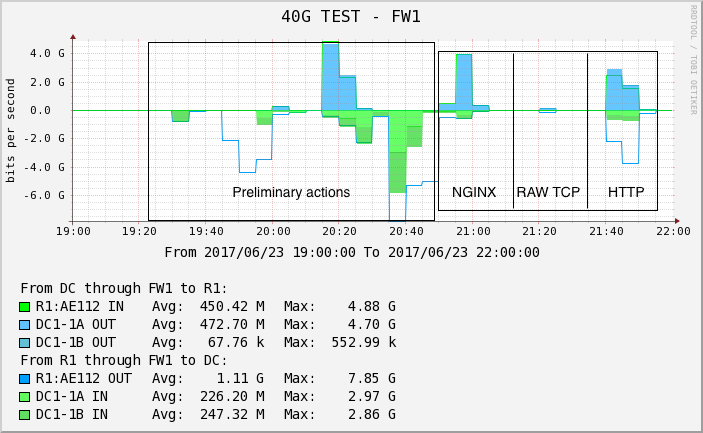
\includegraphics[scale=0.5]{images/real-ae112.png}
  \caption{Bandwidth utilization of links between router1, firewall1 and DC1 during the time window of the tests, spikes represent an executed test.}
  \label{fig:testrealusageae112}
\end{figure}

\begin{figure}[H]
  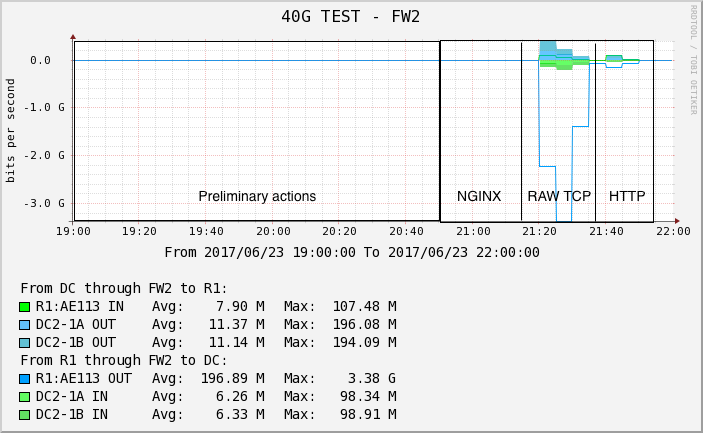
\includegraphics[scale=0.5]{images/real-ae113.png}
  \caption{Bandwidth utilization of links between router1, firewall2 and DC2 during the time window of the test, the spike represents the moment of a fail over to the secondary machine.}
  \label{fig:testrealusageae113}
\end{figure}

The graph in figure \ref{fig:testrealusageae113} displays the generated traffic. When the test started, the active firewall crashed and a failover to the passive machine is the result. Log messages retrieved from connected routers also display BGP session failures from the formerly-active firewall. 
This graph also displays the difference between traffic sent from the router to the firewall and the traffic received by the downstream switch. 
Input is 3Gb/s and output is in the range of 200 - 300 Mb/s. The firewall was configured to accept all the traffic from the source range of the test server inside the network.

The firewalls are not capable of handling this amount of sessions per second. Due to time restrictions this test could not be performed again to pinpoint the maximum number of sessions.  
When the test was finished, the firewalls recovered. \\ 

At 21:40 the third and last test is started between server and client, again both running WARP. 
Generating the maximum amount of HTTP sessions using 32GB of memory and all available cores.
Generating a GET request and responding with a 200-OK message from the server running WARP instead of NGINX.  
From the experimental phase of this research it is known that WARP is capable of handling more requests per second than NGINX can. This last test is executed to find the limits of intermediate hardware when HTTP sessions are opened up in a fast rate.
Message sizes for this tests are : 64, 256, 512, 1024 and 2048 bytes. Request and response size are equal. 
With the information from the benchmark in chapter \ref{ch:experiments} the limitations of client and server are known. 
From test two it is known the firewalls cannot handle the load  when to many sessions per second come in. The same behavior is expected during this last test.
Figure \ref{fig:testrealusageae112} shows 4Gb/s going into the firewall and only 500Mb/s of HTTP traffic arriving at the other side.
This means that the firewall was not able to handle the amount of new sessions per second which caused it to stop functioning \cite{forti3200}. 
Management sessions broke down and traffic got lost as the figures display. \\

In a real world scenario like the one we used in these test, limitations can be revealed by executing the test described in chapter \ref{ch:method}. 
The unexpected fail over of the firewall when one million session were sent to the destination server is a perfect example of finding the weakest link in the chain.
It was not the bandwidth nor the amount of packets per second that made the firewall crash, but the amount of sessions are the limitation for tests two and three. 

This proves that DPDK and WARP can be utilized to perform end-to-end application layer testing. 
WARP can generate the load to a service in order to see if the service can handle the expected load. WARP can also be used to find the limitation of the infrastructure towards an application.

